\chapter{Landauer's cost at body temperature}\label{ch:landauer}

Thermal noise is the unit of measure in this Part. Cytosine methylation is written and erased by enzymes, it is stable once written, and its pattern
across the genome carries information about what a cell is and what state it is in~\cite{Sanchez2016}. That makes it an information-writing process in
the sense of Landauer~\cite{Landauer1961}, with a least cost per irreversible operation of $\kB T\ln2$. This chapter fixes the numbers that follow from
that statement at body temperature, places the cell beside two engineered substrates on one dimensionless ratio, and sets out where the
reading of this Part agrees with, and where it parts from, the earlier information thermodynamics of methylation.

\section{The cost of one bit}

At $\Tb=310.15$~K,
\begin{equation}
  e_{\mathrm{bit}}=\kB\Tb\ln2=(1.380649\times10^{-23})(310.15)(0.693147)
  =2.968\times10^{-21}\ \mathrm{J},
  \label{eq:ebit}
\end{equation}
or $1.787$~kJ per mole of bits. \calc{} This is the least free energy that must be dissipated to
make one irreversible binary commitment at body temperature. It is not the cost the cell actually
pays; it is the floor under whatever mechanism the cell uses.

\section{The Mahaffey number}

The cell's currency for irreversible work is ATP. Under cytosolic conditions the free energy of
hydrolysis is about $\dGATP\approx54$~kJ\,mol$^{-1}$, larger than the standard value of
30.5~kJ\,mol$^{-1}$ because the cell holds ATP far from equilibrium with ADP and
phosphate~\cite{Nelson2017}. The ratio of that drive to the thermal quantum is
\begin{equation}
  M=\frac{\dGATP}{R\Tb}=\frac{54\,000}{8.314462618\times310.15}=20.94 .
  \label{eq:M}
\end{equation}
\calc

\begin{definition}[Mahaffey number]
For any system that drives irreversible events with energy $\Edrive$ per event against a thermal
environment at temperature $T$,
\[
  M=\frac{\Edrive}{\kB T}.
\]
It is dimensionless and fixed by the physics of the drive: the energy a substrate spends per irreversible write, in units of the thermal noise
quantum at its operating temperature. For the cell $M=20.94$; present CMOS logic runs a few hundred $\kB T$ per switch
(Chapter~\ref{ch:cmos}).
\end{definition}

Two points of usage matter. First, $M$ is a constant of the cell's chemistry, not a reading of a
person: every human cell at 37~\textdegree C has the same $M$. Second, $M$ is defined without a
factor of $\ln2$, so that it counts the drive in thermal quanta $\kB T$ rather than in bits. The number of Landauer bits that one ATP can
pay for is then a separate quantity,
\begin{equation}
  \frac{M}{\ln2}=\frac{\dGATP}{N_A\,\kB\Tb\ln2}=30.21 .
  \label{eq:bitsperATP}
\end{equation}
\calc{} Figure~\ref{fig:budget} sets the two side by side.

\paragraph{A ratio, not a rate.} $M$ is energy over energy, and it has no time in it. A metabolic rate is energy per unit time: it
rises with exercise, fever and illness, and a calorimeter measures it. $M$ would have the same value in a cell frozen at one instant.
The gauge of Chapter~\ref{ch:gauge} reads neither quantity. It reads the methylation pattern itself, on the sites that make a cell
what it is. \derived{} for the units. That a cell can turn over ATP quickly with a well-held pattern, or slowly with a poorly held
one, is \interp.

\paragraph{Three quantities, not two.} It is tempting to call ATP the information and temperature the noise. Three quantities are
involved. Thermal motion, on the scale $R\Tb$, randomizes marks; it is the denominator of $M$. The free energy of ATP is what the
cell spends to hold its pattern against that motion; it is the numerator. The pattern, which sites are held methylated and which are
held unmethylated, is the information, and it is what an array or a sequencing read records. The first two are the same in every
human cell at 37~\textdegree C. \derived{} The third differs from one cell type to the next: on single molecules the healthy copy
error ranges 0.024--0.042 across 56 cell types (Chapter~\ref{ch:iama}). \measured{} That is why a cell is read against the healthy
reading of its own type and not against one number for the body.

\begin{figure}[htbp]\centering
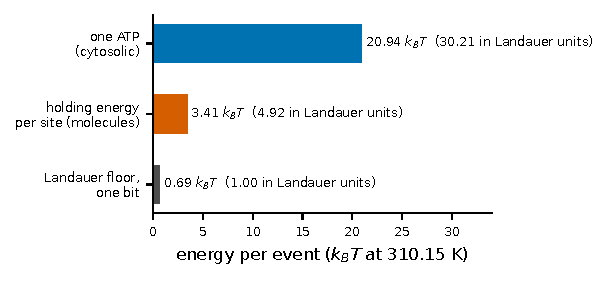
\includegraphics[width=0.62\textwidth]{figures/part6/fig_cell_budget.pdf}
\caption{Energy per event at body temperature in units of $\kB T$: the Landauer floor for one bit ($\ln2=0.69$), the holding energy per
site measured on single molecules ($3.41$, Section~\ref{sec:p4holding}) and one ATP hydrolysis under cytosolic conditions ($M=20.94$). In
Landauer units, $E/\kB T\ln2$, the same three are 1.00, 4.92 and 30.21. \calc{} (the holding energy is \measured)}
\label{fig:budget}
\end{figure}

\section{The cell beside a transistor and a qubit}\label{sec:p4operating}

The same ratio places engineered information-writing substrates, whose inputs are fully measured, relative to the thermal noise at which they
run. Table~\ref{tab:p4operating} and Figure~\ref{fig:p4operating} set the cell beside a CMOS logic transistor and an aluminum transmon.

\begin{table}[htbp]\centering\small
\caption{The dimensionless operating ratio $M=\Edrive/\kB T$ for three information-writing substrates, with its value in Landauer units
$M/\ln2$. For the transmon the drive is taken as $\Edrive=\Delta_{\rm Al}\ln2$ and the operating temperature as the gap temperature
$T_{\rm gap}=\Delta_{\rm Al}/\kB$; the gap cancels and $M=\ln2$. The chip value is the whole-chip average of Chapter~\ref{ch:cmos}. \calc}
\label{tab:p4operating}
\begin{tabular}{@{}llllr@{}}\toprule
substrate & $\Edrive$ & $T$ & $M$ & $M/\ln2$ \\\midrule
CMOS logic, AMD Ryzen 9 9950X & $\mathrm{TDP}/(N_{\rm trans}f)$ & 348.15~K & 399--411 & 576--593 \\
human cell nucleus & $\dGATP$ & 310~K & 20.94 & 30.21 \\
aluminum transmon & $\Delta_{\rm Al}\ln2$ & $\Delta_{\rm Al}/\kB$ & $\ln2=0.693$ & 1 \\\bottomrule
\end{tabular}
\end{table}

The transmon line is the saturated case: at its gap temperature the drive is exactly one Landauer bit,
\begin{equation}
  M_{\rm transmon}=\frac{\Delta_{\rm Al}\ln2}{\kB\,(\Delta_{\rm Al}/\kB)}=\ln2,\qquad \frac{M_{\rm transmon}}{\ln2}=1 ,
  \label{eq:Mtransmon}
\end{equation}
\derived{} the case superconducting-qubit engineering approaches by cooling until $\kB T$ is the only energy scale left. The cell cannot cool.
At 310~K it spends $20.94\,\kB T$ per ATP, 30.2 times the Landauer floor of one bit. \calc

\begin{figure}[htbp]\centering
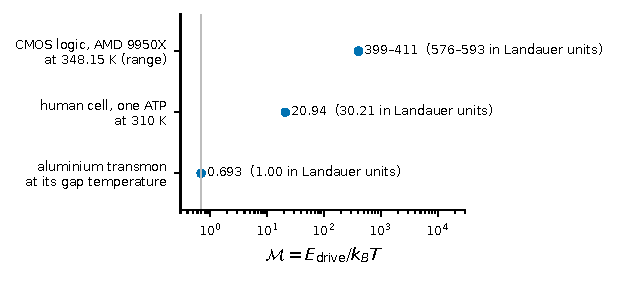
\includegraphics[width=0.62\textwidth]{figures/part6/fig_p4_02_operating.pdf}
\caption{The operating ratio $M=\Edrive/\kB T$ of Table~\ref{tab:p4operating} on a log axis; the vertical line is the Landauer floor, $M=\ln2$.
The chip's point is labeled with the range set by its two published transistor counts. \calc}
\label{fig:p4operating}
\end{figure}

$M$ and the healthy reference entropy of a cell are different quantities. $M$ is one number for the substrate, fixed by biochemistry. The
reference entropy is one number per cell type, in bits, fixed by measuring purified healthy cells of that type (Chapter~\ref{ch:meta}). The
claim of this section is modest and arithmetical: the ratio engineers use to place a transistor or a qubit relative to thermal noise places the
cell at about 21, and the healthy reference of a cell type is a statement about how that cell holds its written state at that ratio. \calc{}
Why $\kB T$ is the right unit is argued from IAM's Law in Part~\ref{part:1} (Chapter~\ref{ch:iams_law}); nothing in the measurements of this Part
depends on that argument.

\section{What a methyl mark costs the cell}

The methyl group on cytosine comes from $S$-adenosylmethionine (SAM). Methionine adenosyltransferase
builds SAM from methionine and ATP and releases all three phosphates, as pyrophosphate and
phosphate; pyrophosphate is then hydrolyzed. The methyl transfer leaves $S$-adenosylhomocysteine,
which is hydrolyzed and recycled to methionine through the folate and B$_{12}$ cycle, at further
cost. So each methyl mark costs the cell at least one ATP-equivalent, and in practice more.
\begin{equation}
  \frac{\text{chemical cost of one mark}}{\text{Landauer floor of one bit}}\gtrsim\frac{M}{\ln2}\approx30 .
  \label{eq:markmargin}
\end{equation}
\calc{} The cell pays at least thirty times the physical minimum for each bit it writes. That factor
is the \emph{cellular margin}: headroom between what the physics requires and what the chemistry
spends.

\section{The floor for one copy of the methylome}

At each S phase the cell copies its methylation pattern onto the new strands. DNMT1, recruited by
UHRF1 to hemimethylated CpGs at the replication fork, restores the methyl group opposite each
methylated parental CpG~\cite{Bostick2007,Sharif2007}. Every CpG of the new strand is a binary decision, methylated or not, so the
Landauer floor counts every CpG. The CpG index of the human reference genome (hg19) holds $N=28{,}217{,}448$ CpGs, and the floor for one
copy is
\begin{equation}
  E_{\mathrm{floor}}=N\,\kB\Tb\ln2=2.822\times10^{7}\times2.968\times10^{-21}
  =8.38\times10^{-14}\ \mathrm{J},
  \label{eq:efloor}
\end{equation}
equal to $9.3\times10^5$ ATP at 54~kJ\,mol$^{-1}$, or $1.0\times10^6$ at 50~kJ\,mol$^{-1}$. \calc{} Figure~\ref{fig:divfloor} shows the floor
for other ways of counting the sites.

\begin{figure}[htbp]\centering
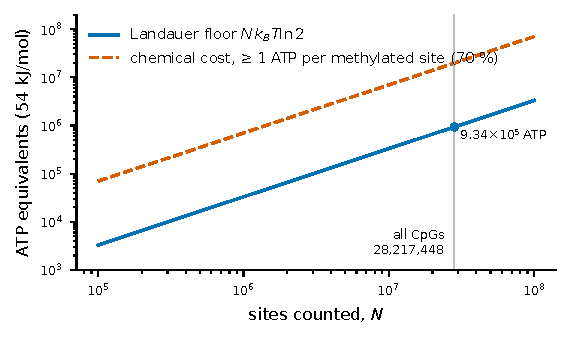
\includegraphics[width=0.62\textwidth]{figures/part6/fig_division_floor.pdf}
\caption{Landauer floor for one full rewrite of the methylation pattern, in ATP equivalents
($\dGATP=54$~kJ\,mol$^{-1}$), as a function of how many sites are counted (solid), and the chemical cost of writing a methyl group at the
70~\% of sites that are methylated, at one ATP each (dashed). At all 28,217,448 CpGs the floor is $9.34\times10^5$ ATP. \calc}
\label{fig:divfloor}
\end{figure}

\begin{checkbox}
A growing mammalian cell of about $3000\,\mu\mathrm{m}^3$ turns over ATP at a rate of order $10^9$ per second~\cite{Milo2015}. Over a
24-hour cycle that is of order $10^{14}$ ATP. In a typical somatic cell roughly 70~\% of CpGs are methylated, so one copy writes about
$2.0\times10^7$ methyl groups at one ATP or more each: a fraction of order $10^{-7}$ of the cell's energy budget. The Landauer floor of
the copy, $9.3\times10^5$ ATP, is about twenty times smaller again: thirty per written mark (Eq.~\eqref{eq:markmargin}), times the 70~\% of
decisions that need a mark. \calc{} \emph{Energy is not what limits a cell's methylation.} Whatever makes a cell lose or gain entropy on its
identity sites, it is not that the cell cannot afford the ATP. This is the first place where a naive reading of ``the cell cannot pay its
cost'' fails, and the book returns to it in Chapter~\ref{ch:floorbreach}.
\end{checkbox}

\section{Margin per write, and fidelity per write}

If total energy does not bind, what does? The answer the numbers point to is \emph{fidelity per
write}. A copying process that discriminates the right outcome from the wrong one by a free-energy
difference $\Delta\Delta G$ makes errors with probability of order $e^{-\Delta\Delta G/\kB T}$
(the equilibrium-discrimination limit; kinetic proofreading can do better at extra
cost~\cite{Hopfield1974}).

Hairpin-bisulfite measurements at CpG sites of the human \emph{FMR1} promoter give site-specific, per-division
maintenance efficiencies of 0.90--0.98~\cite{Genereux2005}. \observed{} A maintenance failure rate of 2--10~\%
corresponds to
\[
  \frac{\Delta\Delta G}{\kB T}=\ln\frac{1}{0.02\text{--}0.10}=2.3\text{--}3.9 .
\]
\calc{} The cell spends about $21\,\kB T$ per ATP and realizes a discrimination of about $2$--$4\,\kB T$
per methylation decision. The large gap between the two is where the physics of methylation
lives.

\paragraph{The holding energy, measured on molecules.}\label{sec:p4holding} The same quantity can be read directly on single DNA molecules.
On read-level whole-genome bisulfite data from a public atlas of sorted healthy human cells~\cite{Loyfer2023}, 153 of its 205 samples
grouped here into 56 cell types (the atlas paper groups its 205 samples into 39), the copy error $\varepsilon$
(an unmethylated CpG isolated between methylated neighbors, on molecules that are otherwise methylated) gives, through
$E_{\rm hold}=\kB T\ln[(1-\varepsilon)/\varepsilon]$, a holding energy of $3.41\pm0.12\,\kB T$ per site, range 3.13--3.71, in
every cell type. \measured{} In Landauer units that is $3.41/\ln2=4.92$. \calc{} As a fraction of one ATP it is
\begin{equation}
  \phi=\frac{E_{\rm hold}}{M\,\kB T}=0.163\pm0.006 .
  \label{eq:phi}
\end{equation}
The value sits inside the range implied by the copying enzyme's own measured preference for hemimethylated over unmethylated
sites in vitro, 7--21-fold for the purified human enzyme~\cite{Pradhan1999} and 80-fold on average across flanking
sequences~\cite{Adam2023}, which by Hopfield's relation~\cite{Hopfield1974} is $\kB T\ln(\text{selectivity})=1.9$--$4.4\,\kB T$. \calc
That is a consistency check from independent biochemistry, not a confirmation. Chapter~\ref{ch:iama} turns
Eq.~\eqref{eq:phi} into the floor of the gauge. A cell's methylation pattern is not a static record: it is a steady state between a writing
process of finite fidelity and the cell's own divisions and demethylation, and its entropy on any
set of loci is set by that balance. Chapter~\ref{ch:surface} makes this precise.

\section{Where this stands: the information thermodynamics of methylation}\label{sec:sanchez}

That cytosine methylation obeys Landauer's bound is not new. Sanchez and Mackenzie~\cite{Sanchez2016} treated a change of methylation
status at a genomic region as an information-processing operation. With $p_i$ the methylation level at cytosine $i$, the per-site Shannon
entropy
\begin{equation}
  H(C_i)=-p_i\log_2p_i-(1-p_i)\log_2(1-p_i)
  \label{eq:sanchezH}
\end{equation}
measures the uncertainty of methylation status at tissue level. The information processed in a region $R$ is the change $I_R$ of
$\sum_{i\in R}H(C_i)$, and by Landauer's principle the least energy dissipated to process it is
\begin{equation}
  E_R=I_R\,\kB T\ln2 .
  \label{eq:sanchezER}
\end{equation}
\derived{} (from Landauer's principle, given Eq.~\eqref{eq:sanchezH}) They showed that the distribution of $E_R$ across genomic regions, the
background of methylation change induced by thermal fluctuation, is well described by a Weibull distribution (a member of the
generalized-gamma family) whose scale parameter recovers the persistence length of DNA, 39--67~nm, from methylome data alone, and that
regulatory signal can be discriminated from that background by signal-detection theory. \observed{} Their 2019 paper~\cite{Sanchez2019}
turned this into a method, the MethylIT package: an information divergence (Hellinger) of each sample from a reference built from control
individuals, a per-sample Weibull or gamma fit yielding a critical value, and a classifier-derived optimal cutoff separating disease-induced
from background differentially methylated positions. \observed

Three things are taken from that work as established and built on. (i) $\kB T\ln2$ is the correct physical anchor for methylation as an
information-writing process. (ii) Thermal fluctuations produce a genuine statistical background in methylation level that any analysis must
account for. (iii) In Sanchez and co-workers' terms, proper measurement of the methylation signal needs a reference from which divergence is
measured, so that background and signal are measured with ``the same origin of coordinates''~\cite{Sanchez2019}.

The approaches part at exactly that point. In MethylIT the origin of coordinates is the centroid of a control group in the study at hand, a
reference re-established for every study. Here the question is whether the origin can instead be fixed by the physics and by the healthy cell of
the same kind, so that one specimen can be read with no other specimen in the room (Chapters~\ref{ch:meta} and~\ref{ch:iama}). The question was reached independently, from the thermodynamics of bound systems rather than from
epigenetics; their 2016 paper was read only after the first reference values had been frozen. It is cited because it is
peer-reviewed physics that the methylome obeys Landauer's bound, and so that a reader who knows MethylIT sees precisely where the two
approaches agree and where they part.

Two clarifications for such a reader. First, a reading here is a ratio of entropies to a fixed reference, not a divergence between two samples.
It carries no information about which sites moved, only how far the cell as a whole sits from its healthy entropy; where on the genome the
departures sit is a separate map (Chapters~\ref{ch:cscore} and~\ref{ch:sky}). Second, whole blood and tissue are mixtures. Before any cell is
read, the specimen's composition is solved against purified references (Chapter~\ref{ch:separation}), and a reading is reported only for cell
types found present above a presence floor.

\paragraph{One filters, one calibrates.} Both approaches rest on $\kB T\ln2$. Sanchez and Mackenzie use it to model the thermal background of
methylation change and, in MethylIT, to filter that background away, so that regulatory sites can be found and classified against a control
reference. This Part uses it as the unit of measure, and asks how far above the thermal floor a cell holds its written state, against a
reference fixed once by physics and the healthy cell. The two are complementary rather than competing. Their statistical-mechanical background
model is a principled way to ask which identity sites carry regulatory rather than thermal signal, a question answered here by site selection
(Chapter~\ref{ch:identity}); it is the first extension to test. \openprob{} In the other direction, the calibration discipline of
Chapter~\ref{ch:instrument} applies to any absolute methylation measurement, including one built on divergences: a
divergence from a control pool inherits that pool's laboratory and pipeline offset, and on the immune identity sites of 450K arrays that offset,
between raw-IDAT noob processing and the processed reference methylomes, is about $0.075$ in $\beta$. \measured

Three limitations of the comparison should be stated. Their data are whole-genome bisulfite sequencing read counts; the array results here are
statements about arrays. Their signal is a site that moved; a reading here is a cell against its reference, and carries no site-level
information. And their 2016 proposal of a binary methylation ``language'' is not used or evaluated.

\section{Summary}
\begin{center}\small
\begin{tabularx}{\linewidth}{@{}>{\raggedright\arraybackslash}X>{\raggedright\arraybackslash}p{0.36\linewidth}l@{}}\toprule
quantity & value & status \\\midrule
$\kB\Tb\ln2$ & $2.968\times10^{-21}$ J & \calc \\
$M=\dGATP/R\Tb$ & 20.94 & \calc \\
Landauer bits per ATP, $M/\ln2$ & 30.21 & \calc \\
transmon at its gap temperature & $M=\ln2=0.693$; 1 in Landauer units & \derived \\
CMOS, AMD 9950X, whole-chip average & $M=399$--$411$ & \calc \\
floor for all 28,217,448 CpGs & $8.38\times10^{-14}$ J $=9.3\times10^5$ ATP & \calc \\
chemical cost per mark / floor & $\gtrsim30$ & \calc \\
maintenance discrimination & 2--4 $\kB T$ & \calc{} from~\cite{Genereux2005} \\
holding energy on molecules, 56 cell types & $3.41\pm0.12\,\kB T$ (4.92 Landauer units) & \measured \\
$\phi=E_{\rm hold}/M\kB T$ & $0.163\pm0.006$ & \measured \\
pipeline offset on immune identity sites, 450K & $\approx0.075$ in $\beta$ & \measured \\\bottomrule
\end{tabularx}
\end{center}
